\section{Ecken kompatible Paare}

In diesem Abschnitt werden wir uns mit einer zweiten Charakterisierung von SLTRs auf planaren Graphen nach \cite{af15} beschäftigen, die eine Verbindung zwischen Schnyder Woods und FAAs herstellt und so zu einer hinreichenden Bedingung für SLTRs führt. Zum Einstieg folgt die Definition dieses Zusammenhanges.

\begin{definition}[Ecken Kompatibilität]\label{def_coco}
Ein Paar $(\sigma,\phi)$ aus einem Schnyder Labeling $\sigma$ und einem FAA $\phi$ nenne wir \textit{Ecken kompatibel}, falls:
\begin{itemize}
\item [C1] Das Schnyder Labeling $\sigma$ und das FAA $\phi$ nutzen die selben Aufhängungen.
\item [C2] In jedem inneren Gebiet haben die drei Ecken aus $\phi$ drei unterschiedliche Label in $\sigma$.
\end{itemize}
\end{definition}

Der Rest dieses Kapitels wird sich mit dem Beweis beschäftigen, dass zu jedem SLTR (mindestens ein) Ecken kompatibles Paar existiert und das anders herum jedes Ecken kompatible Paar eine SLTR induziert.

\begin{theorem}\label{theo_coco}
Sei G ein planer, intern-3-zusammenhängender Graph mit den Aufhängungen $\{a_1,a_2,a_3\}$. G besitzt eine SLTR, genau dann wenn ein Ecken kompatibles Paar $(\sigma,\phi)$ aus einem Schnyder Labeling $\sigma$ und einem FAA $\phi$ existiert.
\end{theorem}

Wir beweisen zuerst die (deutlich einfachere) Rückrichtung des Theorems. Hier können wir die durch das in Abschnitt \ref{sw} erklärte \textit{face counting} erhaltene Einbettung nutzen, um zu zeigen, dass jeder begrenzende Zykel $\gamma$ genau drei kombinatorisch konvexe Ecken besitzt.

\begin{lemma}\label{lem1}
Sei G ein planer, intern-3-zusammenhängender Graph mit den Aufhängungen $\{a_1,a_2,a_3\}$. Falls ein Paar $(\sigma,\phi)$ aus einem Schnyder Labeling $\sigma$ und einem FAA $\phi$ Ecken kompatibel ist, dann hat jeder begrenzende Zykel $\gamma$ genau drei kombinatorisch konvexe Ecken im Bezug auf $\phi$.
\end{lemma}

\begin{proof}
Sei $\gamma$ ein begrenzender Zykel und $F_{in}$ die Menge der inneren Gebiete von $G$. Seien $\alpha_1=(0,1),\alpha_2=(1,0)$ und $\alpha_3=(0,0)$ drei linear unabhängige Vektoren in $\mathbb{R}^2$. $D$ sei die durch \textit{face counting} erhaltende Zeichnung von $G$ mit den Ecken $\alpha_1,\alpha_2,\alpha_3$. Ein Beispiel einer solchen Zeichnung findet sich in Abbildung \ref{face_counting}. Betrachte nun den begrenzenden Zykel $\gamma$ in $D$. Wir schieben nun, wie in Abbildung \ref{sweeplines1} illustriert, ausgehend von $\alpha_i$ die Geraden $(\alpha_{i+1},\alpha_{i-1})$ über den Graphen. Sei $M_i$ die Menge der zuerst von $(\alpha_{i+1},\alpha_{i-1})$ getroffenen Knoten von $\gamma$ für $i \in (1,2,3)$.

\begin{observation}\label{obs1}
Alle Knoten um ein inneres Gebiet $f$ mit Label $i$ in $f$ werden von der Gerade $(\alpha_{i+1},\alpha_{i-1})$ zum gleichen Zeitpunkt getroffen. Dies folgt direkt aus Eigenschaft W5 (Abschnitt \ref{sw}), da alle Knoten mit dem selben Label in der Zeichnung auf $c_i(\alpha_{i+1},\alpha_{i-1})$ platziert werden.
\end{observation}

\begin{observation}\label{obs2}
Sei $v \in M_i$. Alle Winkel an $v$ im Inneren von $\gamma$ haben das Label $i$. Die Geraden teilen die Winkel um einen Knoten (siehe Abbildung \ref{sweeplines2}). Die Winkel an $v$, die von $a_i$ aus gesehen vollständig auf der anderen Seite von $(\alpha_{i+1},\alpha_{i-1})$ liegen, haben Label $i$.
\end{observation}

\begin{figure}
  \centering
  \begin{minipage}{0.4\textwidth}
  \centering
    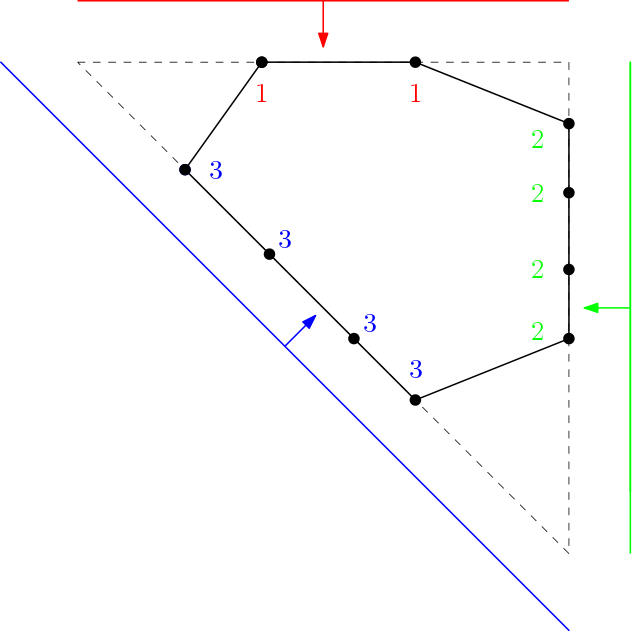
\includegraphics[width=0.9\textwidth]{sweeplines1.png}
    \caption{}
    \label{sweeplines1}
  \end{minipage}
  \hfill
  \begin{minipage}{0.4\textwidth}
  \centering
    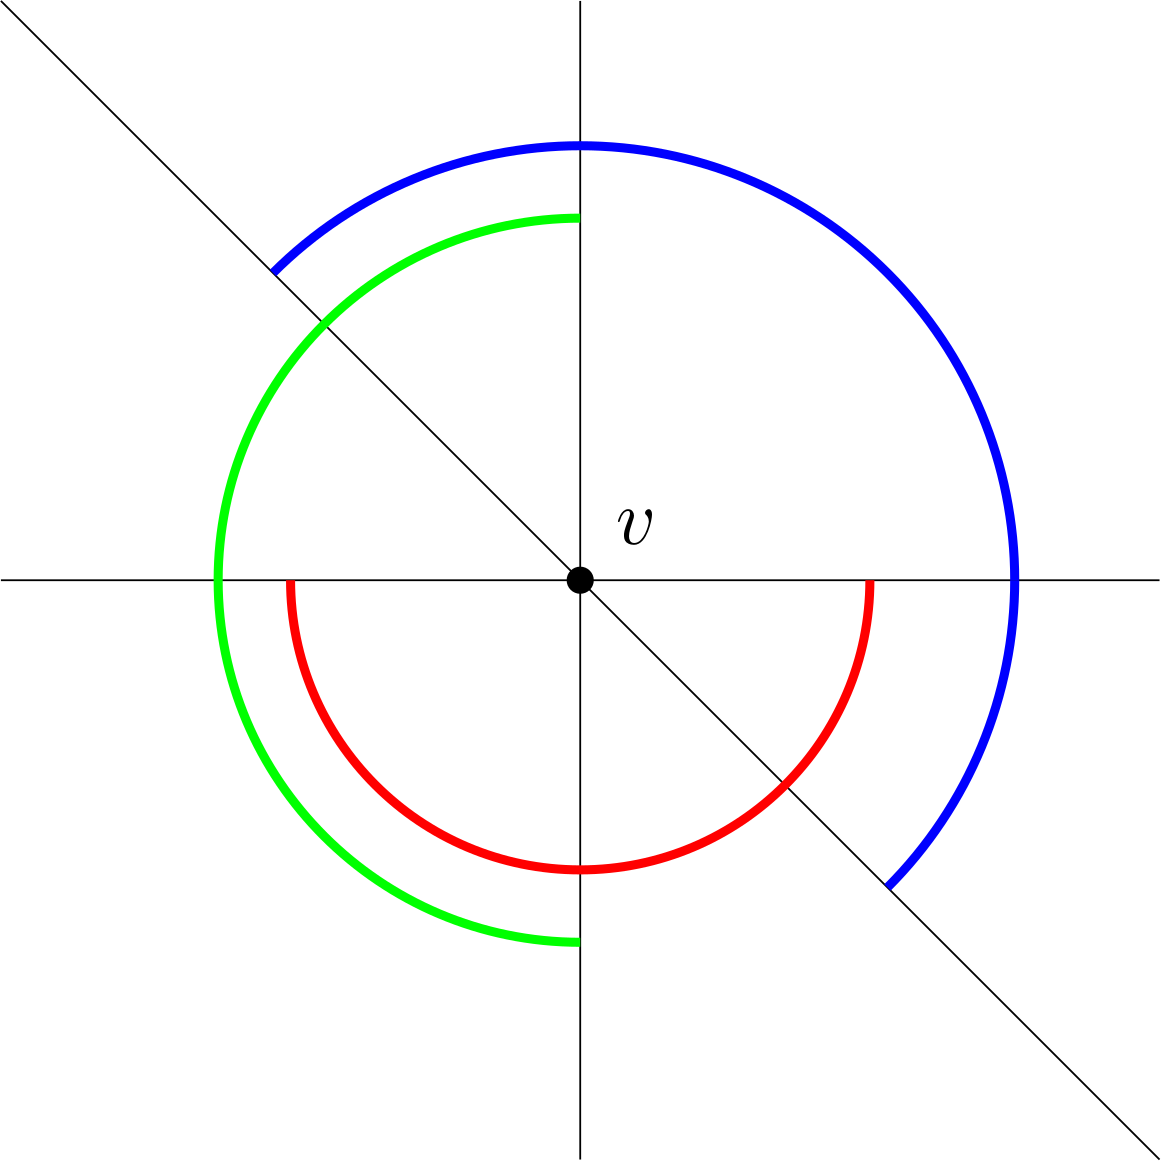
\includegraphics[width=0.9\textwidth]{sweeplines2.png}
    \caption{}
    \label{sweeplines2}
  \end{minipage}
\end{figure}

Nach Beobachtung \ref{obs2} sind die Mengen $M_1,M_2$ und $M_3$ disjunkt. Wir suchen nun nach drei kombinatorisch konvexen Ecken von $\gamma$. Das FAA und das Schnyder Labeling sind Ecken kompatibel und somit hat jedes Gebiet $f \in F_{in}$ einen Winkel mit Label $i$. Also liegt in jeder Menge $M_i$ ein Knoten $v_i$, der vom FAA nicht einem Gebiet innerhalb von $\gamma$ zugewiesen wird. Nehmen wir an $a_i \notin M_i$, denn sonst hätten wir nach E1 eine Ecke gefunden. Da $D$ eine konvexe Zeichnung ist muss $v_i$ einen Nachbarn ausserhalb von $\gamma$ besitzen. Somit liegt $v_i$ auf $\gamma$, ist nicht in $\gamma$ zugewiesen und hat einen Nachbarn ausserhalb von $\gamma$. $v_i$ erfüllt also E2 und somit hat jeder begrenzende Zykel drei kombinatorisch konvexe Ecken (jeweils eine aus jedem $M_i$).
\end{proof}

Zusammen mit Theorem \ref{com_theo} folgt, dass es sich bei dem FAA um ein Gutes-FAA handelt. Somit induziert das Ecken kompatible Paar ein SLTR von $G$.\\

Machen wir uns an den Beweis der Hinrichtung. Zu jedem SLTR können wir ein eindeutiges FAA erstellen indem wir die flachen Winkel der SLTR im FAA zuweisen. Wir müssen also zeigen, dass zu jeder SLTR ein Schnyder Labeling existiert, das zusammen mit dem induzierten FAA ein Ecken kompatibles Paar bildet. Sei $G$ ein planer, intern-3-zusammenhängender Graph mit den Aufhängungen $\{a_1,a_2,a_3\}$, der (mindestens) eine SLTR besitzt. Sei $\Delta$ eine SLTR von $G$ und sei $\phi$ das von $\Delta$ induzierte FAA.

Vor dem nächsten Lemma müssen wir zwei geometrische Objekte einführen. Beispiele finden sich in Abbildung \ref{subdividing_ex}.

\begin{definition}[Unterteilendes Dreieck]
Ein \textit{unterteilendes Dreieck} ist ein Dreieck in der Zeichnung einer SLTR von $G$, sodass gilt:
\begin{itemize}
\item Jeder Knoten auf dem Rand des Dreiecks (der keine Ecke des Dreiecks ist) ist entweder ausserhalb oder innerhalb des Dreiecks zugewiesen
\item Es existiert ein Knoten (der keine Ecke ist), der keine Nachbarn ausserhalb des Dreiecks hat und es existiert ein Knoten (der keine Ecke ist), der keine Nachbarn im Inneren des Dreiecks hat.
\end{itemize}
Dieses Dreieck kann Teile des Randes der Zeichnung beinhalten.
\end{definition}

\begin{definition}[teilendes Segment]
Ein \textit{teilendes Segment} eines SLTR von $G$ ist eine Menge von Kanten $\{e_1, \ldots , e_m\}$, die alle auf einer Gerade liegen, sodass gilt:
\begin{itemize}
\item Die Vereinigung der Kanten trennt die Zeichnung in zwei nichtleere Teile. 
\item Jeder innere Knoten $v$ auf dem Segment ist einem Gebiet zugeordnet, dass zwei Kanten beinhaltet die auf dem Segment liegen. Diese beiden Kanten haben $v$ als Endpunkt.
\end{itemize}
\end{definition}

\begin{figure}[h]
	\centering
	  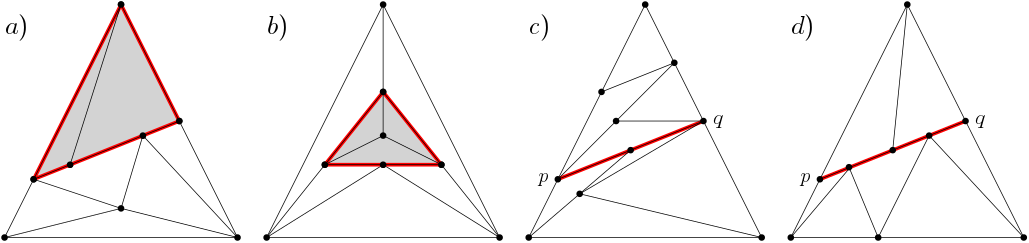
\includegraphics[width=0.9\textwidth]{subdividing_ex.png}
    	\caption{Beispiele von unterteilenden Dreiecken in a) und b) und teilenden Segmenten in c) und d) jeweils in rot.}
    	\label{subdividing_ex}
\end{figure}

Um zu zeigen, dass wir zu jeder SLTR ein passendes Ecken kompatibles Paar $(\sigma,\phi)$ finden führen wir einen Widerspruchsbeweis. Sei $G$, ein kleinstmögliches Gegenbeispiel, zu dem kein Paar existiert. Damit seien hier zuerst die minimale Anzahl an Knoten und darauf folgend die kleinste Anzahl von Kanten gemeint. Sei $\Delta$ eine SLTR von $G$, $\phi$ das induzierte FAA und $a_1,a_2$ und $a_3$ die Aufhängungen von $\Delta$.

Wir zeigen zuerst zwei Eigenschaften von $\Delta$.

\begin{lemma}\label{lem_subtri}
Ein minimales Gegenbeispiel $\Delta$ hat kein unterteilendes Dreieck.
\end{lemma}

\begin{proof}
Nehmen wir an, dass $\Delta$ ein unterteilendes Dreieck mit den Ecken $(a,b,c)$ beinhaltet. Seien $\Delta_1$ und $\Delta_2$ die Teile von $\Delta$ die alles ausserhalb (1) und innerhalb (2) des Dreiecks beinhalten. Der Rand des Dreiecks $(a,b,c)$ liegt in beiden Teilen.

Wir ersetzen Knoten auf dem Rand des Dreiecks die Grad zwei in $\Delta_i$ haben mit einer Kante zwischen ihren Nachbarn. Somit sind $\Delta_1$ und $\Delta_2$ SLTRs mit weniger Knoten als $\Delta$. Da sie weniger Knoten haben als $\Delta$ können sie keine Gegenbeispiele sein und es existieren zu den SLTRs $\Delta_i$ Ecken kompatible Paare $(\sigma_i,\phi_i)$, wobei die $\phi_i$ die induzierten FAAs von $\Delta_i$ sind. Setzen wir die Paare zusammen kommen wir zu einen Widerspruch. Die Ecken $a,b,c$ sind die Aufhängungen von $\Delta_2$. Wir wählen ihre Label so, dass sie mit den inneren Labeln des (jetzt) leeren Dreiecks in $\Delta_1$ übereinstimmen\footnote{Wir können die Label beliebig umbenennen, ohne das Schnyder Labeling zu verändern.}. Die auf diese Weise kombinierten Schnyder Labelings $\sigma_1$ und $\sigma_2$ ergeben ein Schnyder Labeling auf $G$. Die FAAs $\phi_1$ und $\phi_2$ ergeben zusammen, wenn wir die Zuweisungen an den äusseren Knoten von $\Delta_2$ und den am leeren Dreieck liegenden Knoten von $\Delta_1$ anpassen, ein FAA $\phi$ für $G$. Somit folgt die Ecken Kompatibilität aus der Tatsache, dass $(\sigma_1,\phi_1)$ und $(\sigma_2,\phi_2)$ Ecken kompatibel sind. Die SLTR $\Delta$ induziert somit ein Ecken kompatibles Paar und kann kein Gegenbeispiel sein. Somit kann $\Delta$ kein unterteilendes Dreieck haben.
\end{proof} 

\begin{lemma}
Ein minimales Gegenbeispiel $\Delta$ hat kein teilendes Segment.
\end{lemma}

\begin{remark}
Insbesondere bedeutet dies, dass in $\Delta$ für jede Aufhängung $deg(a_i) \geq 3$ gelten muss.
\end{remark}

\begin{proof}
Angenommen $\Delta$ hat ein teilendes Segment mit den Endpunkten $p$ und $q$. Falls auf beiden Seiten des teilenden Segmentes eine Aufhängung mit Grad größer als zwei liegt, dann wird ein unterteilendes Segment in $\Delta$ induziert (siehe Abbildung \ref{subdividing_ex} d)). Falls es sich bei $p$ oder $q$ um eine Aufhängung handelt, bedeutet dies ebenfalls, dass ein unterteilendes Dreieck existiert\footnote{Falls auf der einen Seite des Segmentes nur die Aufhängung $a_i$ liegt wird kein unterteilendes Dreieck impliziert. Jedoch existiert dann mit $\Delta' = \Delta \backslash \{s_1\}$ ein kleineres SLTR (welches dann kein Gegenbeispiel ist) und aus diesem lässt sich ein Ecken kompatibles Paar für $\Delta$ bauen.}. Somit können wir annehmen, dass das teilende Segment zwischen $p$ und $q$ die Aufhängung $s_1$ von Grad zwei abtrennt. $p,q$ und $s_1$ bilden also ein Dreieck. Wir betrachten zwei Fälle. Entweder das teilende Segment besteht nur aus der Kante $(p,q)$ (Fall 1) oder es existiert mindestens ein weiterer Knoten auf dem Segment (Fall 2).\\

\underline{1. Fall}: Falls $p$ Grad drei und dritten Nachbar $p'$ hat, dann muss die Kante $(p',q)$ existieren und $(s_1,q,p)$ ist ein unterteilendes Dreieck mit der inneren Kante $(p,q)$. Dies ist ein Widerspruch zu Lemma \ref{lem_subtri} und es folgt $deg(p),deg(q) \geq 4$. Da $deg(s_1) = 2$ gelten muss und $G$ intern-3-zusammenhängend ist liegt $s_1$ alleine auf der einen Seite des Segments und alle anderen Nachbarn von $p$ und $q$ auf der anderen. 
Wir behaupten, dass mindestens eine der Kanten $(s_1,p)$ und $(s_1,q)$ kontrahierbar ist, sodass der resultierende Graph ein SLTR besitzt. Die Zuweisungen bleiben, bist auf bei $p$ und $q$, gleich (siehe Abbildung \ref{lem3_1}, b)). Dieser Schritt ist nicht trivial. Es könnte passieren, dass in beiden Fällen keine SLTR existiert. Wir nutzen als Kriterium die begrenzenden Zykel aus Definition \ref{def_ccc}. Damit beide Kontraktionen nicht zum erwünschten Ergebnis führen, müssen zwei begrenzende Zykel $\gamma_v,\gamma_w$ mit genau drei kombinatorisch konvexen Ecken, $p,q$ und $v$ respektive $w$, existieren (siehe Abbildung \ref{lem3_1}, c)). Nur dann induziert die Kontraktion von $(s_1,p)$ und $(s_1,q)$ einen Zykel mit nur zwei Ecken. 

Dieser Fall kann aber nicht auftreten. Seien $v,w$ die Ecken dieser Zykel. Dann existieren Pfade $P_{p\to w}$ und $P_{q\to w}$. Diese Pfade sind Teil vom $\gamma_v$ und $\gamma_w$ und enthalten somit keine Ecken ausser an den Enden. Die Winkel an diesen Pfaden im Inneren der Zykel sind somit $\geq \pi$. Sei $z$ der Knoten an dem sich $P_{p\to w}$ und $P_{q\to w}$ kreuzen. Da $z$ keine Ecke sein kann muss er auf beiden Zyklen $\gamma_v,\gamma_w$  zugewiesen sein. Somit müsste der Winkel im inneren der Zykel der an $z$ von $P_{p\to w}$ und $P_{q\to w}$ eingeschlossen wird mindesten $\pi$ sein. Dies ist ein Widerspruch zur Annahme das $\Delta$ eine SLTR ist (siehe Abbildung \ref{lem3_1}, c)).

\begin{figure}[h]
	\centering
	  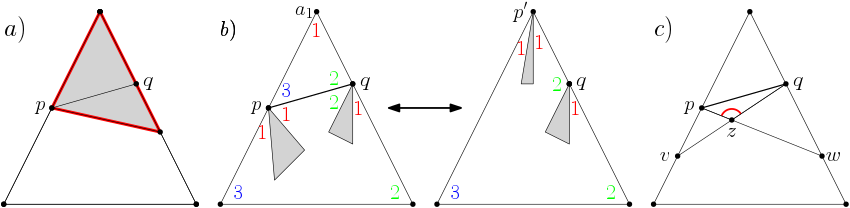
\includegraphics[width=0.9\textwidth]{lem3_1.png}
    	\caption{a) Unterteilendes Dreieck bei Grad 3. b) Kantenkontraktion der Kante $(s_1,p)$. c) Die Pfade die bei der Kontraktion von $(s_1,p)$ oder $(s_1,q)$ Degeneriertheit induzieren.}
    	\label{lem3_1}
\end{figure}

Es kann also mindestens eine der Kanten kontrahiert werden. Sei $(s_1,p)$ diese Kante und $G'$ der Graph der durch Kontraktion von $(s_1,p)$ und das Löschen von $(p,q)$ entsteht. Wir erhalten das FAA $\phi'$ durch löschen der Zuweisung von $p$ aus $\phi$. Der Knoten $q$ ist weiterhin dem äusseren Gebiet zugewiesen. Da $G'$ weniger Knoten als $G$ hat ist es kein Gegenbeispiel und wir erhalten einen Schnyder Labeling $\sigma'$, das zusammen mit $\phi'$ ein Ecken kompatibles Paar bildet. Wir können $\phi'$ zu einem Labeling von $G$ erweitern indem wir, beginnend bei $s_1$, im Uhrzeigersinn die Label $1,2$ und $3$ im Gebiet $s_1,q,p$ einfügen. Dieses Labeling ist offensichtlich Ecken kompatibel. \\

\underline{2. Fall}: 

\end{proof} 

